\exer{Tri à bulles}
\setcounter{numques}{0}


Le tri à bulles est un algorithme de tri classique. Son principe est simple, et il est très
facile à implémenter.
On considère un tableau de nombres $T$, de taille $N$. L'algorithme parcourt le tableau, et dès que deux éléments consécutifs ne sont pas ordonnés, les échange. Après un premier passage, on voit que le plus grand élément se situe bien en dernière position. On peut donc recommencer un tel passage, en s'arrêtant à l'avant-dernier élément, et ainsi de suite.

Au $i$-ème passage on fait remonter le $i$-ème plus grand élément du tableau à sa position définitive, un peu à la manière de bulles qu'on ferait remonter à la surface d'un liquide, d'où le nom d'algorithme de tri à bulles.

\begin{center}
    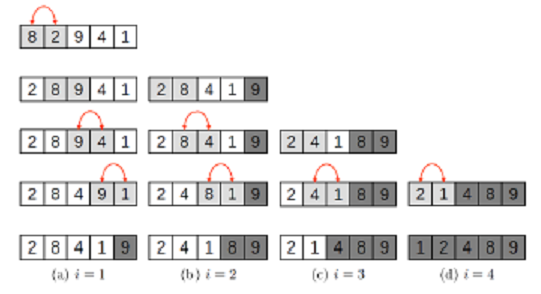
\includegraphics{TriBulles.png}
\end{center}

\question{Appliquer l'algorithme de tri à Bulles <<à la main>> au tableau ci-dessous:} 

$$\begin{array}{|c|c|c|c|c|c|}
    \hline2& 1 & 6 & 9 & 8 & 4 \\
    \hline\end{array}$$

\question{Écrire une fonction \texttt{est\_trie(T)} qui renvoie \texttt{True} ou \texttt{False} selon que le tableau \texttt{T} est trié ou pas.}

\question{Écrire une fonction \texttt{TriBulles(T)} triant le tableau \texttt{T} par l'algorithme de tri à
bulles \footnote{cette fonction doit agir sur place concernant le tableau \texttt{T} ie doit le modifier par effet de bord.}}


\question{Vérifier que la fonction ci-dessus est correcte en utilisant la fonction \texttt{EstTrie} sur des  tableaux de nombres aléatoires. On rappelle que la bibliothèque random permet de créer des nombres aléatoires. \texttt{random.randint(a,b)} renvoie un entier aléatoire compris entre $a$ et $b$.}

\question{Montrer que la complexité est quadratique (notion définie dans I)}

\question{Écrire une fonction améliorée \texttt{TriBulles2(T)} qui sort de la fonction dès que le tableau a été parcouru sans faire d'échange (auquel cas, il est trié et donc inutile de continuer).}

\question{Une variante du tri à bulles est le tri cocktail: il consiste à changer de direction à chaque passage. Lors
du premier parcours, on se déplace du début du tableau vers la fin. Puis lors du second parcours on
part de la fin du tableau pour arriver au début. À la troisième itération on part du début et ainsi de
suite ... C'est une légère amélioration car il permet non seulement aux plus grands éléments de
migrer vers la fin de la série mais également aux plus petits éléments de migrer vers le début.}

\question{\'Ecrire une fonction \texttt{TriCocktail(T)} qui étant donné un tableau \texttt{T} le renvoie trié selon la méthode du tri cocktail.}

\question{Justifier en quoi cette variante peut être intéressante selon le type de tableau à trier mais vérifier néanmoins que la complexité reste quadratique.}

%\end{multicols}
